\documentclass[OPS,lsstdraft,authoryear,toc]{lsstdoc}
% GENERATED FILE -- edit this in the Makefile
\newcommand{\lsstDocType}{RTN}
\newcommand{\lsstDocNum}{098}
\newcommand{\vcsRevision}{f21e126}
\newcommand{\vcsDate}{2025-05-29}


% Package imports go here.

% Local commands go here.

%If you want glossaries
%\input{aglossary.tex}
%\makeglossaries

\title{Target-of-Opportunity Operations During the Science Verification Surveys}

% This can write metadata into the PDF.
% Update keywords and author information as necessary.
% \hypersetup{
%     pdftitle={Rubin ToO operations and procedures},
%     pdfauthor={Sean MacBride,
%                Tiago Ribeiro
               
%                }}

% Optional subtitle
% \setDocSubtitle{A subtitle}

\author{%
Sean MacBride
}

\setDocRef{RTN-098}
\setDocUpstreamLocation{\url{https://github.com/lsst/rtn-098}}

\date{\vcsDate}

% Optional: name of the document's curator
% \setDocCurator{The Curator of this Document}

\setDocAbstract{%
We describe the procedures and workflows for Target-of-Opportunity observations during commissioning and the science verification surveys. We describe the global state of the Rubin ToO system, the workflow during the early commissioning period, the responses to real and mock alerts, and lessons learned from this period. 
}

% Change history defined here.
% Order: oldest first.
% Fields: VERSION, DATE, DESCRIPTION, OWNER NAME.
% See LPM-51 for version number policy.
\setDocChangeRecord{%
  \addtohist{1}{2025-05-30}{Unreleased.}{Sean MacBride}
}


\begin{document}

% Create the title page.
\maketitle
% Frequently for a technote we do not want a title page  uncomment this to remove the title page and changelog.
% use \mkshorttitle to remove the extra pages
\section{Introduction}\label{sec:introduction}
The LSST covers a wide swath of unique science cases and observation types. Rubin Observatory will enable many scientific discoveries, especially target-of-opportunity (ToO) observations during the early commissioning period. 

Rubin Observatory is uniquely positioned to lead ToO observations through the 2020's and beyond due to it's unique technical capabilities. The $\textasciitilde10\deg^2$ field-of-view of the Rubin optical system allow ToO observations to survey a wide area, while the single-visit depth of the LSST-Camera allows single observations to observe the southern sky for faint transient phenomena. The combination of the large FOV and deep observations make Rubin Observatory an ideal tool for discovery of ToO phenomena.

The Rubin ToO program encompasses 3\% of the LSST, and includes GW, high-energy neutrino, potentially hazardous asteroids, and other time-sensitive astrophysical phenomena as different targets. Each target has a different observing strategy based on observing conditions, the conditions of the astrophysical event, and other parameters. The observing strategies are the product of community input, and were revised in 2024 (\cite{RubinToO2024}). These recommendations were accepted by the survey cadence optimization committee in January 2025 (\cite{PSTN-056}).

While other components of the LSST are not limited by the specific time of observation, ToO is uniquely in that the confirmation of a ToO counterpart requires rapid observations, ranging from mere minutes of alert receipt to hours. The different nature of observations requires different workflows, communication channels, and operations to ensure that ToO observations are valuable to the LSST. 

In the forthcoming sections, we describe the state of the Rubin ToO system (section \ref{sec:sysOverview}), the workflow during the science verification period (section \ref{sec:workflow}), the responses to mock and real alerts (section \ref{sec:ToOEvents}), and lessons learned from the early commissioning and science verification period (section \ref{sec:LessonsLearned}).
\newpage
\section{Systems Overview}\label{sec:sysOverview}
The Rubin ToO system is composed of five distinct components, each responsible for a different aspect of ToO operations and observations.

\begin{figure}
    \centering
    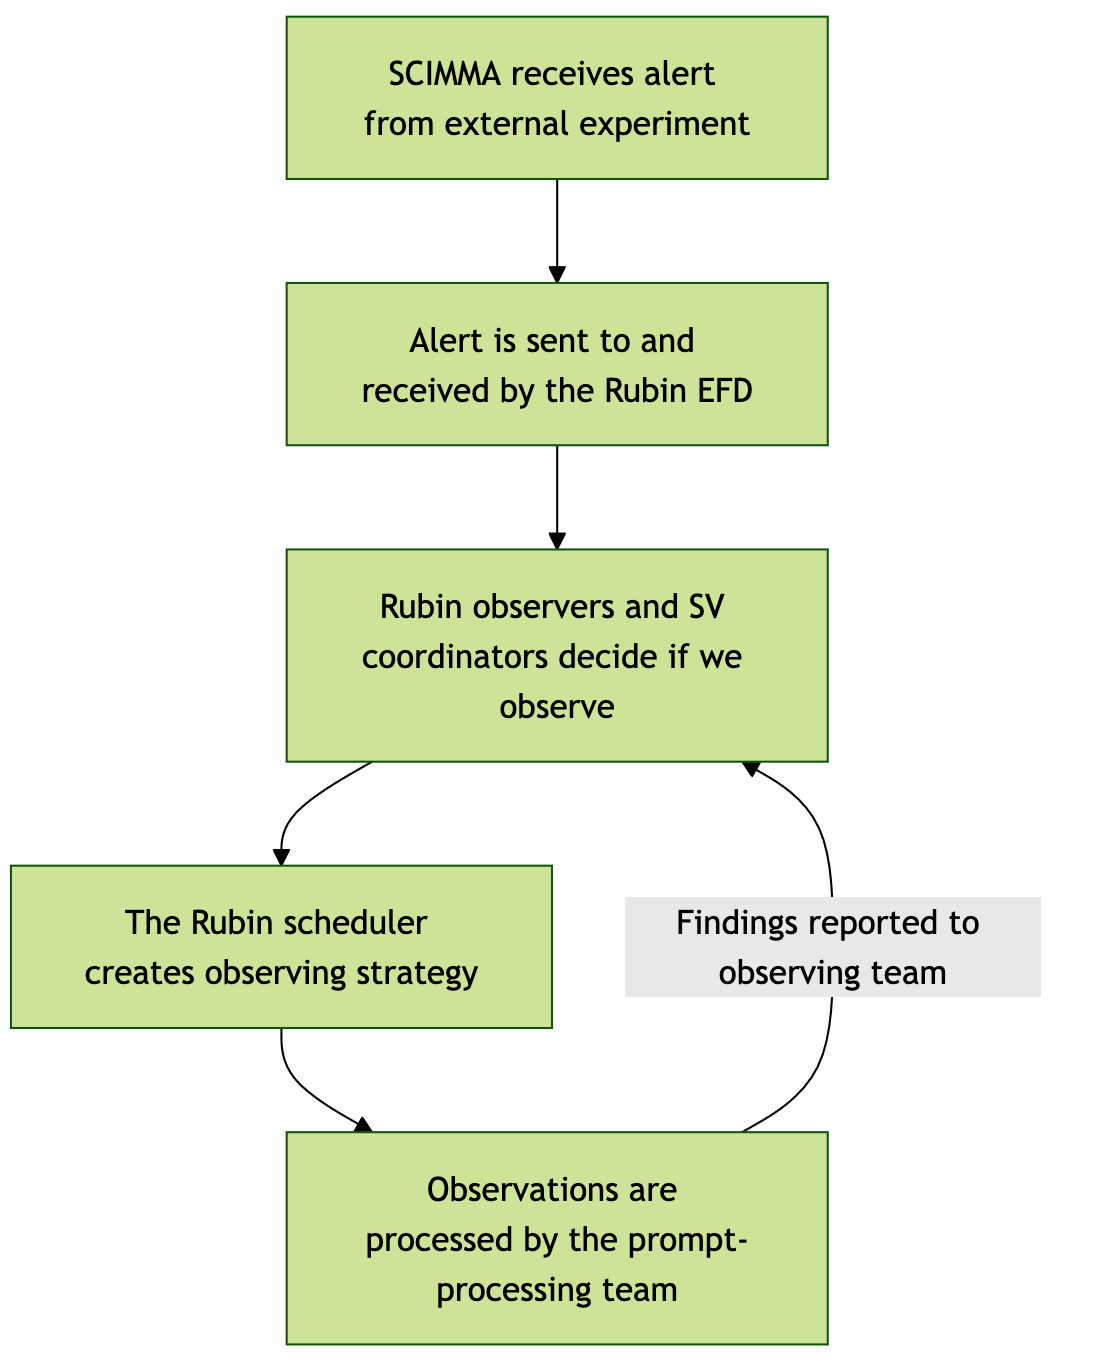
\includegraphics[width=0.6\linewidth]{figures/workflowDiagram.png}
    \caption{The general workflow during the SV period, with the five separate teams and their main responsibilities listed.}
    \label{fig:workflowDiagram}
\end{figure}

\subsection{Incoming alert stream}\label{subsec:alertStream}

The Rubin ToO system starts at the incoming alert stream. The incoming alert stream is responsible for parsing alerts from external experiments and sending them to Rubin infrastructure.

Rubin Observatory considers ToO alerts from a variety of astrophysical phenomena and experiments, including 

\begin{itemize}
    \item \textbf{Gravitational waves:} LIGO-Virgo-KAGRA (LVK) Collaboration
    \item \textbf{High energy neutrinos:} IceCube Neutrino Observatory
    \item \textbf{Potentially hazardous objects:} The NASA Jet Propulsion Laboratory (JPL) Scout and JPL Sentry experiments
    \item \textbf{Galactic supernovae:} The Supernova Early Warning System (SNEWS) and the Super-Kamiokande (Super-K) experiment
    \item \textbf{Lensed GRBs:} LVK and the Neil Gehrels Swift Observatory
\end{itemize}

All incoming alerts are handled by Scalable Cyberinfrastructure to support Multi-Messenger Astrophysics (SCiMMA) HopSkotch. Alerts are received from different experiments before being assessed for alert quality. Alerts of a certain quality are then passed to Rubin infrastructure. In this way, all alerts that arrive at Rubin infrastructure are high quality alerts worthy of follow-up. This enables future revisions of Rubin observing strategy related to ToO to be developed internal to the Rubin Scheduler.

Alert quality for Rubin observations is set by the Rubin science community, who developed a set of criteria for ToO observations in their 2024 recommendation (\cite{RubinToO2024}). This recommendation has been adopted by SCiMMA to ensure the EFD and Rubin scheduler do not need to perform additional checks of alert quality.

\subsection{Engineering facility database}\label{subsec:EFD}

The Rubin engineering facility database (EFD) hosts telemetry and information about every Rubin Observatory component that interacts with middleware. For ToO purposes, this includes SCiMMA alerts. These alerts are received at the summit, including skymap information for the alerts. 

The Scheduler Commandable SAL Component (CSC) collects telemetry from the EFD and hands them over to the Driver, which formats it in a way the scheduling algorithm understands. By using a general purpose interface for collecting and passing telemetry from the EFD to the scheduling algorithm, it allows us to easily add new data sources as long as the data is in the EFD. This flexible design supports the SCiMMA alert stream, but also manual alert information added by observing specialists or other ToO scientists to the EFD (\cite{TSTN-035}). 

\subsection{The Rubin Scheduler}\label{subsec:Scheduler}

At Rubin Observatory, the software that decides when to observe for the LSST is distributed by the \verb|rubin_scheduler| software package. In the \verb|rubin_scheduler| software package, the Feature Based Scheduler (FBS) module encodes the current best approach to achieving these objectives for LSST. The \verb|rubin_scheduler| also contains a simulation mode to generate simulated surveys at high speed, which is useful in simulating different conditions and ToO alerts. 

In section \ref{subsec:Scheduler verification}, references to the Rubin scheduler refer to the simulation mode. In all other sections, mentions of the Rubin Scheduler refer to the FBS implementation within the scheduler CSC, taking images in support of the LSST for the Rubin Observatory.

\begin{table}[]
\centering
\begin{tabular}{|l|l|}
\hline
\textbf{Rubin Scheduler ToO configuration} & \textbf{Strategy from \cite{RubinToO2024}} \\ \hline \hline
GW\_case\_B                         & GW, neutron star component, gold ($\Omega <100\deg^2$)                                             \\ \hline
GW\_case\_C                         & GW, Unidentified source, gold ($\Omega <100\deg^2$)                                   \\ \hline
GW\_case\_D                         & GW, neutron star component, silver ($\Omega <500\deg^2$)                                           \\ \hline
GW\_case\_E                         & GW, Unidentified source, silver ($\Omega <500\deg^2$)                                 \\ \hline
BBH\_case\_A                        & GW, Binary black-hole, dark time, nearby event                                     \\ \hline
BBH\_case\_B                        & GW, Binary black-hole, dark time, distant event                                      \\ \hline
BBH\_case\_C                        & GW, Binary black-hole, bright time                                         \\ \hline
GW\_case\_large                     & GW, large skymaps ($\Omega>500\deg^2$)                                    \\ \hline
lensed\_BNS\_case\_A                & Lensed BNS, $\sim900\deg^2$ skymap                                      \\ \hline
lensed\_BNS\_case\_B                & Lensed BNS, $\sim15\deg^2$ skymap                                       \\ \hline
neutrino and neutrino\_u            & High energy neutrino event                                            \\ \hline
SSO\_night and SSO\_twilight                       & Potentially hazardous asteroid                                           \\ \hline
SN\_Galactic                        & Galactic supernova                                  \\ \hline
Lensed\_GRB                         & Lensed GRB                                          \\ \hline
\end{tabular}
\caption{The strategy naming used in the Rubin Scheduler (left) to execute the community observing strategy recommendations (right) from \cite{RubinToO2024}.}
\label{table:ToOStrategies_sched}
\end{table}

SCiMMA alerts passed to the EFD will have metadata associated with them that denotes the alert type. This piece of metadata is passed to the Rubin scheduler to execute the appropriate strategy, as listed in table \ref{table:ToOStrategies_sched}.

GW observing strategies are differentiated by the 90\% confidence interval area ($\Omega$) from LVK alerts. Unidentified GW sources and NS component sources of similar skymap size (i.e. gold or silver) follow identical strategy. Binary black-hole event strategy is differentiated by the distance of the event and the observing conditions (dark or bright time). All strategies except for large GW skymaps and lensed GRBs have been tested and verified in the Rubin Scheduler (see section \ref{subsubsec:SVRequiredValidation}-\ref{subsubsec:SVOptionalValidation}). Large GW skymaps require specific coordination with the SCOC to cover the area, and lensed GRBs do not have an explicit strategy recommendation in \cite{RubinToO2024}.

\subsection{The Prompt Processing Pipeline}\label{subsec:PP}

Alerts generated by the LSST prompt processing pipeline are LSST’s real-time data product. For prompt-processing to function at full capacity, template coverage of the sky must exist in the region of interest. In the commissioning and early operations era, templates will not be available in many areas, and hence standard alert processing will likely not be used to disseminate candidates. 

Where LSST templates exist, standard LSST processing can proceed as normal, and is currently operating. In regions of insufficient or uncovered template coverage, custom processing will be required. A team of Rubin staff with experience in difference-imaging analysis has been assembled to support on-call processing of ToO areas that are insufficiently covered by existing Rubin templates.

In the case of insufficient Rubin template coverage, two options exist for custom image processing:

\begin{itemize}
    \item \textbf{Difference imaging with external template sources:} template coverage exists from other southern-sky galaxy surveys. The best instrument for alternative template sources is DECam, and the feasibility of template generation with DECam is currently being evaluated.
    \item \textbf{Self-templating:} By taking images over multiple epochs, it is possible to pursue a ToO with a fast evolving lightcurve by observing rapid changes in photometry. The epoch of observation would need to be modified for the ToO to maximize the probability of detecting the variable lightcurve. 
\end{itemize}

Both methods are available to the on-call processing team, and the method of choice will be pursued based on the existing template coverage and alert type of the ToO.

\subsection{The Observing and Science Validation teams}\label{subsec:ObsSVTeams}

In a non-commissioning environment, ToO observations are automated with minimal intervention by observers or ToO scientists. In the era of early Rubin operations, this is not the case. Owing to the commissioning of other Rubin Observatory systems and minimal Rubin template coverage in early operations, ToO observations will require significant intervention and support from the Rubin science community and the prompt-processing groups. 

In line with the recommendations from the SCOC (\cite{PSTN-056}), a ToO advisory committee has been formed. The aim of this committee is to assess the viability of pursuing a ToO during the early operations period. The decision to pursue a particular ToO event, in no particular order, is based upon the following criteria:

\begin{enumerate}
    \item The preparedness of the Observatory to respond to a ToO
    \item The scientific impact of a Rubin-led discovery
    \item The level of disruption to the SV surveys
\end{enumerate}

The ToO advisory committee is composed of Rubin Observatory members with a wide range of expertise. The current committee members are:

\begin{itemize}

    \item Sean MacBride - Rubin ToO coordinator
    \item Zeljko Ivezic - Rubin Construction Project Director
    \item Bob Blum - Rubin Operations Director
    \item Keith Bechtol - System Verification and Validation Scientist
    \item Robert Lupton - Commissioning scientist
    \item Yousuke Utsumi - ToO Scientist and Camera expert
    \item Eric Bellm - Prompt processing lead
    \item Federica Bianco - Deputy project scientist
    \item Tiago Ribeiro - Scheduler scientist and software architect
    \item Shreya Anand - Rubin-LVK Liaison
    \item Deep Chatterjee - LVK Liaison
\end{itemize}
% \newpage
% \section{Existing Bottlenecks}\label{sec:existingBottlenecks}
% \subsection{Incoming alert stream}\label{subsec:alertStream Bottleneck}

\subsection{Engineering facility database}\label{subsec:EFD Bottleneck}

\subsection{The Rubin Scheduler}\label{subsec:Scheduler Bottleneck}

\subsection{The Observing and Science Validation teams}\label{subsec:ObsSVTeams Bottleneck}

\subsection{The Prompt Processing Pipeline}\label{subsec:PP Bottleneck}

\subsection{Resulting data}\label{subsec:resultingData Bottleneck}
\newpage
% \section{Workflow during SV}\label{sec:workflow}
% The workflow during SV will be highly fluid, and subject to change due to lessons learned from testing, early mock ToO responses, and the first ToO triggers with Vera Rubin Observatory. Presented below is the best guess for an efficient and productive ToO response during the SV period.
% \newpage
\section{Tests and ToO Responses}\label{sec:ToOEvents}
\subsection{Alert 1}\label{subsec:alert1}

\newpage
\section{Lessons learned from SV testing}\label{sec:LessonsLearned}
\input{LessonsLearned.tex}

\appendix
% Include all the relevant bib files.
% https://lsst-texmf.lsst.io/lsstdoc.html#bibliographies
\newpage
\section{References} \label{sec:bib}
\renewcommand{\refname}{} % Suppress default Bibliography section
\bibliography{local,lsst,lsst-dm,refs_ads,refs,books}

\newpage
% Make sure lsst-texmf/bin/generateAcronyms.py is in your path
\section{Acronyms} \label{sec:acronyms}
\addtocounter{table}{-1}
\begin{longtable}{p{0.145\textwidth}p{0.8\textwidth}}\hline
\textbf{Acronym} & \textbf{Description}  \\\hline

OPS & Operations \\\hline
RTN & Rubin Technical Note \\\hline
SV & Science Validation \\\hline
ToO & Target of Opportunity \\\hline
\end{longtable}







\end{document}
